\documentclass[11pt]{report}
\usepackage[utf8]{inputenc}
\usepackage{tikz}
\usepackage{a4wide}
\usepackage{algorithm}
\usepackage{algpseudocode}
\usepackage{fancyhdr}
\usepackage{amsmath}
\usepackage{titlesec}
\usepackage{pdfpages}
\usepackage[frenchb]{babel}
\usepackage{graphicx}
\usepackage{amsmath}
\usepackage{amssymb}
%\usepackage{times}


%FONT ANCIEN 
% \usepackage{mathrsfs}
% \usepackage{fourier}
\usepackage{lmodern}
\usepackage[T1]{fontenc}

\usepackage{hhline}
\usepackage{soul}
\usepackage[Glenn]{fncychap}
\usepackage{url}
\usepackage{float}
\usepackage{booktabs} 
\usepackage{enumitem}
\usepackage{xcolor}
\newcommand{\tabitem}{~~\llap{\textbullet}~~}
\usepackage{tcolorbox}
\usepackage{float}
\usepackage{caption}
%\usepackage{indentfirst}% pour tester l'indentationy
\ChNameVar{\fontsize{12}{14}\usefont{OT1}{phv}{m}{n}\bfseries}
\ChNumVar{\fontsize{58}{60}\selectfont\color{black}}
\ChTitleVar{\LARGE\bfseries}
\usepackage[top = 2.5cm, bottom = 2.5cm, left = 3 cm, right = 2.5cm]{geometry}
\usepackage{subcaption}
\usepackage[bottom]{footmisc}

\newtheorem{dfn}{D\'efinition}[section]
\newtheorem{nota}{Notation}
\newtheorem{PseudoDef}[dfn]{Pseudo-D\'efinition}
\newtheorem{prp}[dfn]{Proposition}
\newtheorem{crl}[dfn]{Corollaire}
\newtheorem{thm}[dfn]{Th\'eor\`eme}
\newtheorem{ex}[dfn]{Exemple}
\newtheorem{lmm}[dfn]{Lemme}
\newtheorem{rmq}[dfn]{Remarque}
\newtheorem{prv}[dfn]{Preuve}
\newtheorem{ctrex}[dfn]{Contre-exemple}
\newtheorem{remark}{Remarque }
\newcommand\va{taarif}
\usepackage{url}
\def\UrlBreaks{\do\/\do-}
\usepackage{breakurl}
\usepackage[breaklinks]{hyperref}
\usetikzlibrary{calc} 
\usetikzlibrary{positioning}
% this is my sub-subsection modification (by salim)
% ! remove the red boxes from referenced labels
\hypersetup{hidelinks}

\captionsetup{compatibility=false}



\cfoot{\thepage}

\fancyhead[L]{\quad}

\setlength{\headheight}{21 pt}
\usepackage{hyperref}
\hypersetup{
	backref=true, %permet d'ajouter des liens dans...
	pagebackref=true,%...les bibliographies
	hyperindex=true, %ajoute des liens dans les index.
	colorlinks=false, %colorise les liens
	breaklinks=true, %permet le retour à la ligne dans les liens trop longs
	urlcolor= blue, %couleur des hyperliens
	linkcolor= black, %couleur des liens internes  (blue,red,green,yellow,cyan,magenta)
	bookmarks=true, %créé des signets pour Acrobat
	bookmarksopen=true %si les signets Acrobat sont créés,
	%les afficher complètement.
}

\renewcommand{\labelitemi}{$\bullet$}
\setcounter{tocdepth}{3}
\setcounter{secnumdepth}{3}
\renewcommand\thesubsubsection{\roman{subsubsection}}
\usepackage{minipage-marginpar}


%	pour les algorithmes \Require devient entrées , et \Ensure devient Sorties
\algrenewcommand\algorithmicrequire{\textbf{Entrées:}}
\algrenewcommand\algorithmicensure{\textbf{Sorties:}}

\algdef{SE}{Begin}{End}{\textbf{Begin}}{\textbf{End}}

\title{Titre}
\author{Binome1\_Binome2}
\usetikzlibrary{svg.path}
\usetikzlibrary{shapes.geometric, arrows, decorations.pathmorphing}


\tikzset{basic/.style={draw,fill=none,
                       text badly centered,minimum width=2em}}
\tikzset{input/.style={basic,circle,minimum width=2.5em}}
\tikzset{weights/.style={basic,rectangle,minimum width=2em}}
\tikzset{functions/.style={basic,circle, minimum width=3em}}
\newcommand{\addaxes}{\draw (0em,1em) -- (0em,-1em)
                            (-1em,0em) -- (1em,0em);}
\newcommand{\relu}{\draw[line width=1.5pt] (-1em,0) -- (0,0)
                                (0,0) -- (0.75em,0.75em);}
\newcommand{\stepfunc}{\draw[line width=1.5pt] (0.65em,0.65em) -- (0,0.65em) 
                                    -- (0,-0.65em) -- (-0.65em,-0.65em);}


\begin{document}
	%!	NO TOC SECTIONS
	\newcommand{\notocsection}[1]{%
	\refstepcounter{section}%
	\section*{\thesection \quad #1}}%

	\newcommand{\notocsubsection}[1]{%
	\refstepcounter{subsection}%
	\subsection*{\thesubsection \quad #1}}%


	\newcommand{\notocsubsubsection}[1]{%
	\refstepcounter{subsubsection}%
	\subsubsection*{\thesubsubsection \quad #1}}%

	\renewcommand\thesection{\arabic{section}}
	\renewcommand\thesubsection{\arabic{section}.\arabic{subsection}}
	\renewcommand\theremark{\empty{}}
	\newcommand\subsubsubsection[1]{\paragraph{#1}\mbox{}\\}
	\setcounter{secnumdepth}{4}
	\setcounter{tocdepth}{4}

	\newcommand\subsubsubsubsection[1]{\subparagraph{#1}\mbox{}\\}
	\setcounter{secnumdepth}{5}
	\setcounter{tocdepth}{5}

	\renewcommand\thesubsubsection{\arabic{section}.\arabic{subsection}.\arabic{subsubsection}}
	\renewcommand\theparagraph{\arabic{section}.\arabic{subsection}.\arabic{subsubsection}.\arabic{paragraph}}
	\renewcommand\thesubparagraph{\arabic{section}.\arabic{subsection}.\arabic{subsubsection}.\arabic{paragraph}.\arabic{subparagraph}}

	\begin{titlepage}

% \begin{figure}[htbp]
%  \hbox{
%      
\includegraphics[width=40px]{Logo.png}
%      \hspace*{11.5cm}
%      
\includegraphics[width=40px]{Logo.png}
%   }
% \end{figure}
\begin{figure}[H]
    \centering
    
\includegraphics[scale=0.1]{Logo.png}

    \label{fig:enter-label}
\end{figure}
% \vspace {-1.5cm}

\begin{center}
%%%%%% En-tete


{\bf {\large Sorbonne Université}}\\
{\bf Faculté de Science et d'ingénierie} \\
{ \textbf{D\'epartement Informatique}}\\ \vspace{0.5cm}
%%%%%%%%%%%%%%%%%%%%%%%%%%%%%%%%%%%%%%%%%%%%%%%%%%%%%%%%%
\Huge{\textbf{Rapport du PSTL}} \\ \Large{\textbf{Informatique}} \\\vspace{0.3cm}
\large{\emph{\textbf{Spécialité:} \\ Science et Technologie Logiciel}}\\ \vspace{0.5cm}
\huge{\textbf{Thème}}\\ %\vspace{0.3cm}
\noindent\rule{\textwidth}{1mm}
\Large{\textbf{Génération et réparation d’instances
pour JSON Schema
}}
\noindent\rule{\textwidth}{1mm}
\end{center}
\vspace{0.3cm}
%%%%%%%%%%%%%%%%%%%%%%%%%%%%%%%%%%%%%%%%%%%%%%%%%%%%%%%%
\begin{tabular}{ p{9cm}  p{6cm} }
        \textbf{Encadré par} & \textbf{Réalisé par} \\
        \begin{itemize}
        	\item[\textbullet] { Mohammed-Amine Baazizi }
        	\newline
        	\item[\textbullet] { Lyes Attouche }
        \end{itemize}
        &
        \begin{itemize}
        	\item[\textbullet]{Tabellout Salim}
        	\newline
        	\item[\textbullet]{Tabellout Yanis}
            \newline
        	\item[\textbullet]{Bouzourine Hichem}
        \end{itemize}
\end{tabular}

% \begin{tabular}{ p{9cm}  p{15cm} }
%         \textbf{Membres de jury} \\
%         \begin{itemize}
%         	\item[\textbullet]{\textsc {......}} 
%         	\newline
%         	\item[\textbullet]{\textsc {......}}
%         \end{itemize}
% \end{tabular}

\begin{center}



Soutenu le: \textbf{DD/MM/2024}
\\ 


\end{center}

\end{titlepage}
    % \include{Chapitres/Remerciements/Remerciements.tex}
    % \include{Chapitres/Dedicaces/Dedicace.tex}
	%\maketitle
    %!  TABLE DE CONTENU
\clearpage                       % Otherwise \pagestyle affects the previous page.
{                                % Enclosed in braces so that re-definition is temporary.
  \pagestyle{empty}              % Removes numbers from middle pages.
  \fancypagestyle{plain}         % Re-definition removes numbers from first page.
  {
    \fancyhf{}%                       % Clear all header and footer fields.
    \renewcommand{\headrulewidth}{0pt}% Clear rules (remove these two lines if not desired).
    \renewcommand{\footrulewidth}{0pt}%
  }
  \tableofcontents
  \thispagestyle{empty}          % Removes numbers from last page.
}


%!  TABLE DES FIGURES

\clearpage                       % Otherwise \pagestyle affects the previous page.
{                                % Enclosed in braces so that re-definition is temporary.
  \pagestyle{empty}              % Removes numbers from middle pages.
  \fancypagestyle{plain}         % Re-definition removes numbers from first page.
  {
    \fancyhf{}%                       % Clear all header and footer fields.
    \renewcommand{\headrulewidth}{0pt}% Clear rules (remove these two lines if not desired).
    \renewcommand{\footrulewidth}{0pt}%
  }
  \listoffigures
  \thispagestyle{empty}          % Removes numbers from last page.
}

%\listoftables
	
	
	\pagestyle{fancy}
	\setcounter{page}{1}
	\chapter{Etat de l'art}
% \addcontentsline{toc}{chapter}{Introduction}


    \section{JSON Schema}

        Le JSON Schema \cite{JSON_Schema} est une norme permettant de décrire la structure et les contraintes des données au format JSON (JavaScript Object Notation). Il spécifie la manière dont les données JSON doivent être organisées, les types de données autorisés, les valeurs par défaut, etc.

        \subsection{Utilité du JSON Schema}

            \begin{enumerate}
                \item \textbf{Validation des données :} Il permet de valider si une instance JSON est conforme à un schéma prédéfini, assurant ainsi la qualité et la cohérence des données.
                
                \item \textbf{Documentation :} En décrivant la structure des données attendues, le JSON Schema sert également de documentation explicite pour les utilisateurs et les développeurs.
                
                \item \textbf{Communication :} En partageant un schéma, différentes parties prenantes peuvent avoir une compréhension commune de la structure des données, facilitant ainsi l'échange d'informations.
                
                \item \textbf{Génération de données de test :} Il peut être utilisé pour générer des jeux de données de test conformes au schéma, ce qui est utile lors de la phase de développement et de tests.
            \end{enumerate}

        \subsection{Intégration avec les Objectifs du Projet}

            Dans le cadre du projet, les objectifs visent la génération et la correction d'instances JSON conformes à un schéma initial, tout en minimisant les modifications nécessaires. 

            \begin{enumerate}
                \item \textbf{Validation initiale :} Les générateurs d'instances identifiés dans l'objectif 1 produisent des données JSON à partir des schémas. La première étape consiste à valider ces instances par rapport au JSON Schema, identifiant ainsi les non-conformités.
                
                \item \textbf{Réparation des instances :} L'objectif global du projet est de développer des approches de réparation permettant de minimiser les modifications nécessaires pour rendre une instance non conforme conforme au schéma initial.
                
                \item \textbf{Analyse des erreurs de validation :} L'objectif 4 consiste à étudier le lien entre les erreurs de validation, détectées à l'étape 1, et la distance d'édition entre les instances non conformes et l'instance valide. Cette analyse contribue à une compréhension approfondie des types d'erreurs et guide le processus de réparation.
            \end{enumerate}

    \section{La similarité des documents JSON}
        La similarité des documents JSON est une mesure de la similarité entre deux documents JSON. Elle est généralement utilisée pour comparer des documents JSON qui représentent des objets ou des données similaires.
        \subsection{Approches existantes}
            Une des approches existantes pour calculer la similarité des documents JSON est :
            \begin{itemize}
                \item [\textbullet] \textbf{Approche top-down \cite{JSON_Similarity}:} 
            Cet approche top-down pour un comparateur de similarité dans le contexte JSON consiste à examiner la similarité entre deux structures JSON en commençant par les éléments les plus généraux et en descendant progressivement vers les détails spécifiques. Cela implique une comparaison basée sur la hiérarchie des éléments plutôt que sur les valeurs individuelles. ensuite les valeurs des propriétés et des éléments des deux documents.
            \end{itemize}
        \subsection{Limitations :}
            \begin{enumerate}
                \item \textbf{La structure du document est ignorée :} les approches top-down ignorent la structure du document, ce qui peut conduire à des résultats inexacts.
                \item \textbf{Aucune garantie de qualité n'est donnée :} les approches existantes ne fournissent généralement aucune garantie de qualité pour leurs résultats.
            \end{enumerate}

    \section{JEDI}
        JEDI \cite{JEDI} est un algorithme de calcul de la similarité entre deux documents JSON. Il fonctionne en comparant les deux documents en tant qu'arbres. La similarité entre les deux documents 
        est définie comme le nombre minimum d'opérations d'édition (Ajout, Suppression, Modification) nécessaires pour transformer un arbre en l'autre.
        \begin{figure}[H]
            \centering
            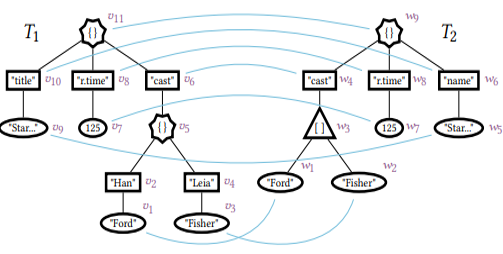
\includegraphics[scale=0.6]{Photos/Tree.png}
            \caption{Exemple de nombre d'opération de transformation}
            \label{fig:tree}
            \cite{JEDI}

        \end{figure}
        \subsection{Représentation d'arbres Json}   
            JEDI \cite{JEDI} introduit la notion \textbf{d'arbre Json} qui est une représentation arborescente d'un document où chaque valeur de l'arbre est représenté par un noeud, nous permettant ainsi d'exploiter 
            certaines propriétés des arbres qui nous sera utile par la suite. La figure \ref{fig:transformation_json_en_arbre} est un exemple sur cette notion.
            \begin{figure}[H]
                \begin{subfigure}[H]{0.45\linewidth}
                    \begin{verbatim}
{
  "title":"star",
  "r.time": 125,
  "cast": {
    "Han": "Ford",
    "Leia": "Fisher"
  }
}
                    \end{verbatim}
                \end{subfigure}
                \begin{subfigure}[H]{0.05\linewidth}
                    $\Longrightarrow$
                \end{subfigure}
                \begin{subfigure}[H]{0.45\linewidth}
                    \begin{center}
                        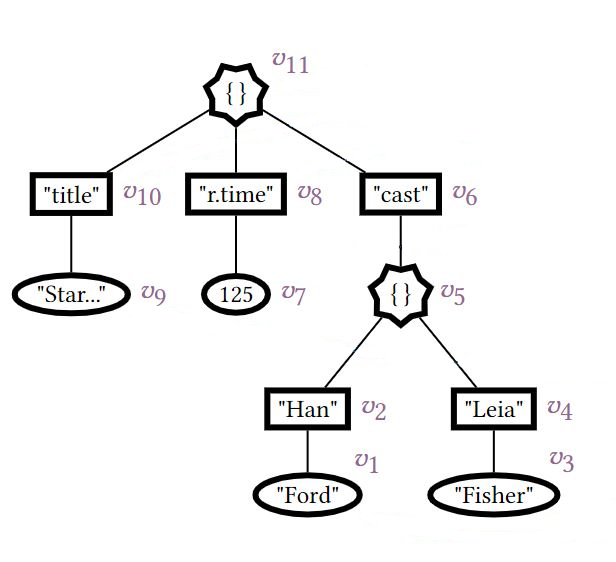
\includegraphics[scale=0.5]{Photos/tree_representation.png}
                    \end{center} 
                \end{subfigure}
                \caption {Transformation d'un document json en arbre Json}
                \label{fig:transformation_json_en_arbre}
            \end{figure}

        \subsection{Distance d'édition (Tree Edit Distance : TED)}
            JEDI permet de calculer la \textbf{distance d'édition} entre \textbf{deux arbres JSON}. On définit \textbf{TED} comme étant le nombre d'opération minimale 
            pour transformer un arbre \textbf{$T_1$} à l'arbre \textbf{$T_2$}. Ces opérations sont :  \emph{ajout, suppression, renomer un noeud} et qui représentent les opérations 
            permettant le \textbf{Json Edit Mapping}, c'est à dire faire correspondre chaque noeud du premier arbre vers le deuxième soit : 
            \begin{itemize}
                \item [\textbullet] Suppression : Les noeuds de $T_1$ qui ne figurent pas dans $T_2$ sont supprimés
                \item [\textbullet] Ajout : Les noeuds de $T_2$ qui ne figurent pas dans $T_1$ sont ajoutés
                \item [\textbullet] Renommer : Les noeuds de $T_1$ qui figurent dans $T_2$ sont renommés
            \end{itemize} 
           
            
            Chaque opération est associé à un coût, sauf le cas de renommer le même noeud \footnote{ Le coût de renommer $v8$ en $w8$ est nulle \ref{fig:tree} car il s'agit du même noeud}
        \subsection{Distance et Matrice d'édition}
            Jedi permet de construire une matrice appelé \textbf{Matrice d'édition} qui sauvegarde la distance d'édition entre chaque noeuds de $T_1$ avec les noeuds de $T_2$, 
            la figure suivante illustre la matrice de l'exemple précédent : 
            \begin{figure}[H]
                \centering
                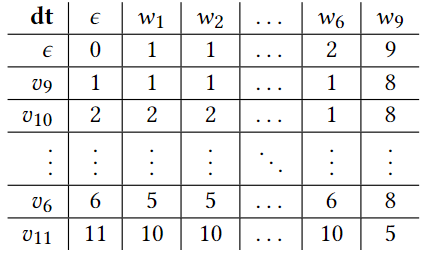
\includegraphics[scale=0.5]{Photos/tree_edit_matrix.PNG}
                \caption{Matrice d'édition entre $T_1$ et $T_2$}
                \label{fig:tree_edit_matrix}
            \end{figure}

            \textbf{\underline{Exemple }}: 
            \begin{figure}[H]
                \centering
                \begin{subfigure}[H]{0.45\linewidth}
                    \begin{verbatim}
{
    "tree":[
        {"height" : 300},
        {"width" : 20}
    ]
}
                    \end{verbatim}
                    \caption{Json $T_1$}
                \end{subfigure}
                \hfill
                \begin{subfigure}[H]{0.45\linewidth}
                    \centering
                    \begin{verbatim}
                        
{
    "tree":[
        300,
        20
    ]
}
                    \end{verbatim}
                    \caption{Json $T_2$}
                \end{subfigure} 
                
            \end{figure}
            \begin{figure}[H]\ContinuedFloat
                \centering
                \begin{tabular}{|c|c|c|c|c|c|}
    \hline
    dt& \{\} & tree & [\hspace{0.2cm}] & 300 & 20 \\ \hline
    \{\} & 4 & 5 & 6 & 8 & 8 \\ \hline
    tree & 5 & 4 & 5 & 7 & 7 \\ \hline
    [\hspace{0.2cm}] & 6 & 5 & 4 & 6 & 6 \\ \hline
    \{\} & 3 & 2 & 2 & 2 & 2 \\ \hline
    height & 3 & 2 & 1 & 1 & 1 \\ \hline
    300 & 4 & 3 & 2 & 0 & 0 \\ \hline
    \{\} & 3 & 2 & 2 & 2 & 2 \\ \hline
    width & 3 & 2 & 1 & 1 & 1 \\ \hline
    20 & 4 & 3 & 2 & 0 & 0 \\ \hline
\end{tabular}
                \caption{Matrice d'édition}
            \end{figure}

            \begin{remark}
                Pour Jedi on ne sauvegarde pas les opérations qu'on fait mais plutôt le coût de modification.
            \end{remark}
            

    \section{Validation d'un schema}


        La \textbf{validation} du JSON Schema est un processus par lequel les données JSON sont vérifiées par rapport à un schéma JSON spécifié pour garantir leur \textbf{conformité aux règles} et aux contraintes définies dans ce schéma comme les règles de typage\cite{Validation}. Le JSON Schema fournit une méthode standardisée pour décrire la structure attendue des données JSON, y compris les types de données, les propriétés requises, les valeurs autorisées, les formats de données et les relations entre les différentes parties des données. \cite{FoundationOfJSONSchema}

        Lorsqu'une validation JSON Schema est effectuée, les données JSON sont \textit{comparées} au schéma correspondant, et toute violation des règles spécifiées dans le schéma est \textit{détectée et signalée}. 


        La validation d'un document par rapport au schéma est toujours en \textbf{PTIME} et peut être résolu en temps linéaire tant que le schéma n'utilise pas de \textit{uniqueItems}.

            \subsection{validation d'un document en PTIME}
            Nous traitons le document restriction par restriction, tout en vérifiant la conformité au sous-schéma correspondant dans S.
            Le temps d’exécution est \textbf{linéaire} car la correspondance à chaque mot-clé du schéma JSON peut être vérifiée en temps linéaire (sauf pour les éléments uniques).
            
            \subsection{Validation d'un document en PTIME-hard}
            On fait la même chose mais on vérifie aussi que les éléments d'un tableau \textit{J} sont uniques, d'abord en \textit{triant} le tableau J.

            La preuve est par réduction du problème de la valeur du circuit monotone
            \subsection*{Exemples de Grammaire JSON Schema}
                
                
            \begin{itemize}
                \item [\textbullet]\textbf{JSDoc :=} {(defs,)? JSch}
                \item [\textbullet]\textbf{Defs :=}         "definitions :{string:{JSch}
                    (,string : {JSch})*
                }
                \item [\textbullet]\textbf{JSch :=} strSch | numSch |intSch | objSch | arrSch | refSch | not | allOf | anyOf | enum
                \item [\textbullet]\textbf{ not :=} "not": {JSch}
            \end{itemize}
            
            


	% \chapter{Etat de l'art}
% \addcontentsline{toc}{chapter}{Introduction}


    \section{JSON Schema}

        Le JSON Schema \cite{JSON_Schema} est une norme permettant de décrire la structure et les contraintes des données au format JSON (JavaScript Object Notation). Il spécifie la manière dont les données JSON doivent être organisées, les types de données autorisés, les valeurs par défaut, etc.

        \subsection{Utilité du JSON Schema}

            \begin{enumerate}
                \item \textbf{Validation des données :} Il permet de valider si une instance JSON est conforme à un schéma prédéfini, assurant ainsi la qualité et la cohérence des données.
                
                \item \textbf{Documentation :} En décrivant la structure des données attendues, le JSON Schema sert également de documentation explicite pour les utilisateurs et les développeurs.
                
                \item \textbf{Communication :} En partageant un schéma, différentes parties prenantes peuvent avoir une compréhension commune de la structure des données, facilitant ainsi l'échange d'informations.
                
                \item \textbf{Génération de données de test :} Il peut être utilisé pour générer des jeux de données de test conformes au schéma, ce qui est utile lors de la phase de développement et de tests.
            \end{enumerate}

        \subsection{Intégration avec les Objectifs du Projet}

            Dans le cadre du projet, les objectifs visent la génération et la correction d'instances JSON conformes à un schéma initial, tout en minimisant les modifications nécessaires. 

            \begin{enumerate}
                \item \textbf{Validation initiale :} Les générateurs d'instances identifiés dans l'objectif 1 produisent des données JSON à partir des schémas. La première étape consiste à valider ces instances par rapport au JSON Schema, identifiant ainsi les non-conformités.
                
                \item \textbf{Réparation des instances :} L'objectif global du projet est de développer des approches de réparation permettant de minimiser les modifications nécessaires pour rendre une instance non conforme conforme au schéma initial.
                
                \item \textbf{Analyse des erreurs de validation :} L'objectif 4 consiste à étudier le lien entre les erreurs de validation, détectées à l'étape 1, et la distance d'édition entre les instances non conformes et l'instance valide. Cette analyse contribue à une compréhension approfondie des types d'erreurs et guide le processus de réparation.
            \end{enumerate}

    \section{La similarité des documents JSON}
        La similarité des documents JSON est une mesure de la similarité entre deux documents JSON. Elle est généralement utilisée pour comparer des documents JSON qui représentent des objets ou des données similaires.
        \subsection{Approches existantes}
            Une des approches existantes pour calculer la similarité des documents JSON est :
            \begin{itemize}
                \item [\textbullet] \textbf{Approche top-down \cite{JSON_Similarity}:} 
            Cet approche top-down pour un comparateur de similarité dans le contexte JSON consiste à examiner la similarité entre deux structures JSON en commençant par les éléments les plus généraux et en descendant progressivement vers les détails spécifiques. Cela implique une comparaison basée sur la hiérarchie des éléments plutôt que sur les valeurs individuelles. ensuite les valeurs des propriétés et des éléments des deux documents.
            \end{itemize}
        \subsection{Limitations :}
            \begin{enumerate}
                \item \textbf{La structure du document est ignorée :} les approches top-down ignorent la structure du document, ce qui peut conduire à des résultats inexacts.
                \item \textbf{Aucune garantie de qualité n'est donnée :} les approches existantes ne fournissent généralement aucune garantie de qualité pour leurs résultats.
            \end{enumerate}

    \section{JEDI}
        JEDI \cite{JEDI} est un algorithme de calcul de la similarité entre deux documents JSON. Il fonctionne en comparant les deux documents en tant qu'arbres. La similarité entre les deux documents 
        est définie comme le nombre minimum d'opérations d'édition (Ajout, Suppression, Modification) nécessaires pour transformer un arbre en l'autre.
        \begin{figure}[H]
            \centering
            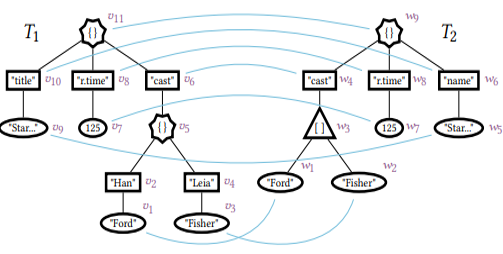
\includegraphics[scale=0.6]{Photos/Tree.png}
            \caption{Exemple de nombre d'opération de transformation}
            \label{fig:tree}
            \cite{JEDI}

        \end{figure}
        \subsection{Représentation d'arbres Json}   
            JEDI \cite{JEDI} introduit la notion \textbf{d'arbre Json} qui est une représentation arborescente d'un document où chaque valeur de l'arbre est représenté par un noeud, nous permettant ainsi d'exploiter 
            certaines propriétés des arbres qui nous sera utile par la suite. La figure \ref{fig:transformation_json_en_arbre} est un exemple sur cette notion.
            \begin{figure}[H]
                \begin{subfigure}[H]{0.45\linewidth}
                    \begin{verbatim}
{
  "title":"star",
  "r.time": 125,
  "cast": {
    "Han": "Ford",
    "Leia": "Fisher"
  }
}
                    \end{verbatim}
                \end{subfigure}
                \begin{subfigure}[H]{0.05\linewidth}
                    $\Longrightarrow$
                \end{subfigure}
                \begin{subfigure}[H]{0.45\linewidth}
                    \begin{center}
                        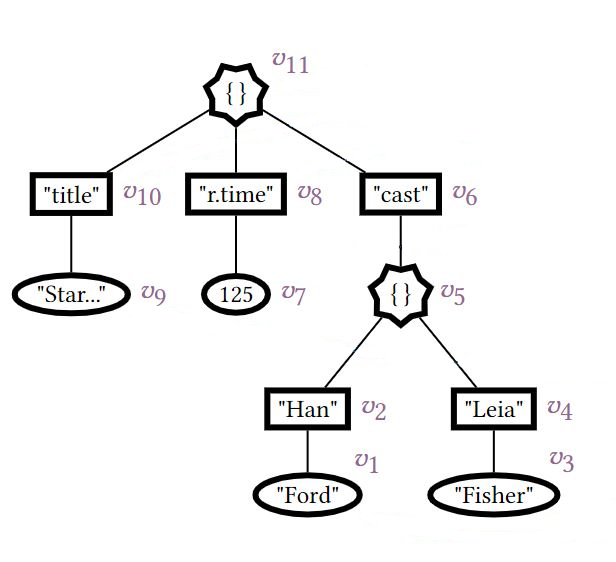
\includegraphics[scale=0.5]{Photos/tree_representation.png}
                    \end{center} 
                \end{subfigure}
                \caption {Transformation d'un document json en arbre Json}
                \label{fig:transformation_json_en_arbre}
            \end{figure}

        \subsection{Distance d'édition (Tree Edit Distance : TED)}
            JEDI permet de calculer la \textbf{distance d'édition} entre \textbf{deux arbres JSON}. On définit \textbf{TED} comme étant le nombre d'opération minimale 
            pour transformer un arbre \textbf{$T_1$} à l'arbre \textbf{$T_2$}. Ces opérations sont :  \emph{ajout, suppression, renomer un noeud} et qui représentent les opérations 
            permettant le \textbf{Json Edit Mapping}, c'est à dire faire correspondre chaque noeud du premier arbre vers le deuxième soit : 
            \begin{itemize}
                \item [\textbullet] Suppression : Les noeuds de $T_1$ qui ne figurent pas dans $T_2$ sont supprimés
                \item [\textbullet] Ajout : Les noeuds de $T_2$ qui ne figurent pas dans $T_1$ sont ajoutés
                \item [\textbullet] Renommer : Les noeuds de $T_1$ qui figurent dans $T_2$ sont renommés
            \end{itemize} 
           
            
            Chaque opération est associé à un coût, sauf le cas de renommer le même noeud \footnote{ Le coût de renommer $v8$ en $w8$ est nulle \ref{fig:tree} car il s'agit du même noeud}
        \subsection{Distance et Matrice d'édition}
            Jedi permet de construire une matrice appelé \textbf{Matrice d'édition} qui sauvegarde la distance d'édition entre chaque noeuds de $T_1$ avec les noeuds de $T_2$, 
            la figure suivante illustre la matrice de l'exemple précédent : 
            \begin{figure}[H]
                \centering
                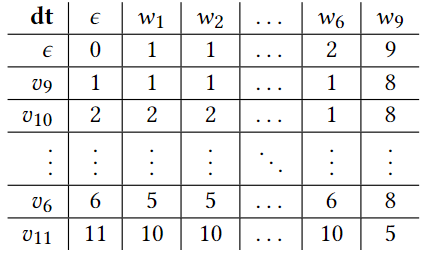
\includegraphics[scale=0.5]{Photos/tree_edit_matrix.PNG}
                \caption{Matrice d'édition entre $T_1$ et $T_2$}
                \label{fig:tree_edit_matrix}
            \end{figure}

            \textbf{\underline{Exemple }}: 
            \begin{figure}[H]
                \centering
                \begin{subfigure}[H]{0.45\linewidth}
                    \begin{verbatim}
{
    "tree":[
        {"height" : 300},
        {"width" : 20}
    ]
}
                    \end{verbatim}
                    \caption{Json $T_1$}
                \end{subfigure}
                \hfill
                \begin{subfigure}[H]{0.45\linewidth}
                    \centering
                    \begin{verbatim}
                        
{
    "tree":[
        300,
        20
    ]
}
                    \end{verbatim}
                    \caption{Json $T_2$}
                \end{subfigure} 
                
            \end{figure}
            \begin{figure}[H]\ContinuedFloat
                \centering
                \begin{tabular}{|c|c|c|c|c|c|}
    \hline
    dt& \{\} & tree & [\hspace{0.2cm}] & 300 & 20 \\ \hline
    \{\} & 4 & 5 & 6 & 8 & 8 \\ \hline
    tree & 5 & 4 & 5 & 7 & 7 \\ \hline
    [\hspace{0.2cm}] & 6 & 5 & 4 & 6 & 6 \\ \hline
    \{\} & 3 & 2 & 2 & 2 & 2 \\ \hline
    height & 3 & 2 & 1 & 1 & 1 \\ \hline
    300 & 4 & 3 & 2 & 0 & 0 \\ \hline
    \{\} & 3 & 2 & 2 & 2 & 2 \\ \hline
    width & 3 & 2 & 1 & 1 & 1 \\ \hline
    20 & 4 & 3 & 2 & 0 & 0 \\ \hline
\end{tabular}
                \caption{Matrice d'édition}
            \end{figure}

            \begin{remark}
                Pour Jedi on ne sauvegarde pas les opérations qu'on fait mais plutôt le coût de modification.
            \end{remark}
            

    \section{Validation d'un schema}


        La \textbf{validation} du JSON Schema est un processus par lequel les données JSON sont vérifiées par rapport à un schéma JSON spécifié pour garantir leur \textbf{conformité aux règles} et aux contraintes définies dans ce schéma comme les règles de typage\cite{Validation}. Le JSON Schema fournit une méthode standardisée pour décrire la structure attendue des données JSON, y compris les types de données, les propriétés requises, les valeurs autorisées, les formats de données et les relations entre les différentes parties des données. \cite{FoundationOfJSONSchema}

        Lorsqu'une validation JSON Schema est effectuée, les données JSON sont \textit{comparées} au schéma correspondant, et toute violation des règles spécifiées dans le schéma est \textit{détectée et signalée}. 


        La validation d'un document par rapport au schéma est toujours en \textbf{PTIME} et peut être résolu en temps linéaire tant que le schéma n'utilise pas de \textit{uniqueItems}.

            \subsection{validation d'un document en PTIME}
            Nous traitons le document restriction par restriction, tout en vérifiant la conformité au sous-schéma correspondant dans S.
            Le temps d’exécution est \textbf{linéaire} car la correspondance à chaque mot-clé du schéma JSON peut être vérifiée en temps linéaire (sauf pour les éléments uniques).
            
            \subsection{Validation d'un document en PTIME-hard}
            On fait la même chose mais on vérifie aussi que les éléments d'un tableau \textit{J} sont uniques, d'abord en \textit{triant} le tableau J.

            La preuve est par réduction du problème de la valeur du circuit monotone
            \subsection*{Exemples de Grammaire JSON Schema}
                
                
            \begin{itemize}
                \item [\textbullet]\textbf{JSDoc :=} {(defs,)? JSch}
                \item [\textbullet]\textbf{Defs :=}         "definitions :{string:{JSch}
                    (,string : {JSch})*
                }
                \item [\textbullet]\textbf{JSch :=} strSch | numSch |intSch | objSch | arrSch | refSch | not | allOf | anyOf | enum
                \item [\textbullet]\textbf{ not :=} "not": {JSch}
            \end{itemize}
            
            


	
	% \include{Chapitres/Chapitre1/chapitre1}
	% \include{Chapitres/Chapitre2/chapitre2}
	% \include{Chapitres/Chapitre3/chapitre3}
	% \include{Chapitres/Chapitre4/conception}
	% \include{Chapitres/Chapitre5/realisation}
	\pagestyle{empty}
	% \include{Chapitres/Conclusion/conclusion}
	\pagestyle{empty}
\clearpage                       
{                                % Enclosed in braces so that re-definition is temporary.
    \pagestyle{empty}              % Removes numbers from middle pages.
    \fancypagestyle{plain}         % Re-definition removes numbers from first page.
    {
        \fancyhf{}%                       % Clear all header and footer fields.
        \renewcommand{\headrulewidth}{0pt}% Clear rules (remove these two lines if not desired).
        \renewcommand{\footrulewidth}{0pt}%
    }
    \bibliographystyle{unsrt}
    \bibliography{bibliographie}
    \thispagestyle{empty}          % Removes numbers from last page.
}
	\appendix
	% \include{Chapitres/AnnexeA/AnnexeA}
	% \include{Chapitres/AnnexeB/AnnexeB} 
	% \include{Chapitres/AnnexeC/AnnexeC} 
	\pagestyle{empty}
	% \include{Chapitres/Résumé/Résumé} 

\end{document}